\chapter{Grundlagen}

\section{Data Mining Frameworks}
Wie in Abschnitt \ref{sec:DataMining} bereits erwähnt, haben sich um das Data Mining drei bekannte Frameworks entwickelt. Diese werden im Nachfolgenden genauer betrachtet. Anschließend findet die Auswahl statt, welches Rahmenwerk Anwendung in dieser Arbeit findet.

\subsection{Knowledge Discovery in Databases (KDD) process model}
Die Bezeichung Knowledge Discovery in Databases wurde hauptsächlich von \citep{fayyad_data_1996} geprägt. Sie beschreiben in ihrer Arbeit ein Problem der 1990er Jahre. Wie auch heute noch, stieg damals die Masse der gespeicherten Daten exponentiell \todo{wirklich "exponentiell"?} an. Die Manuelle Auswertung dieser Datensätze erforderte mehr Arbeitskraft als vorhanden war. \citep[S.~38]{fayyad_data_1996} beschreiben es als "data overload". Deswegen versuchte man, die Prozesse zur Findung von Erkenntnissen zu automatisieren. Daraus hat sich ein Standardvorgehen entwickelt, dass das KDD-Prozessmodell darstellt.
\begin{figure}[h]
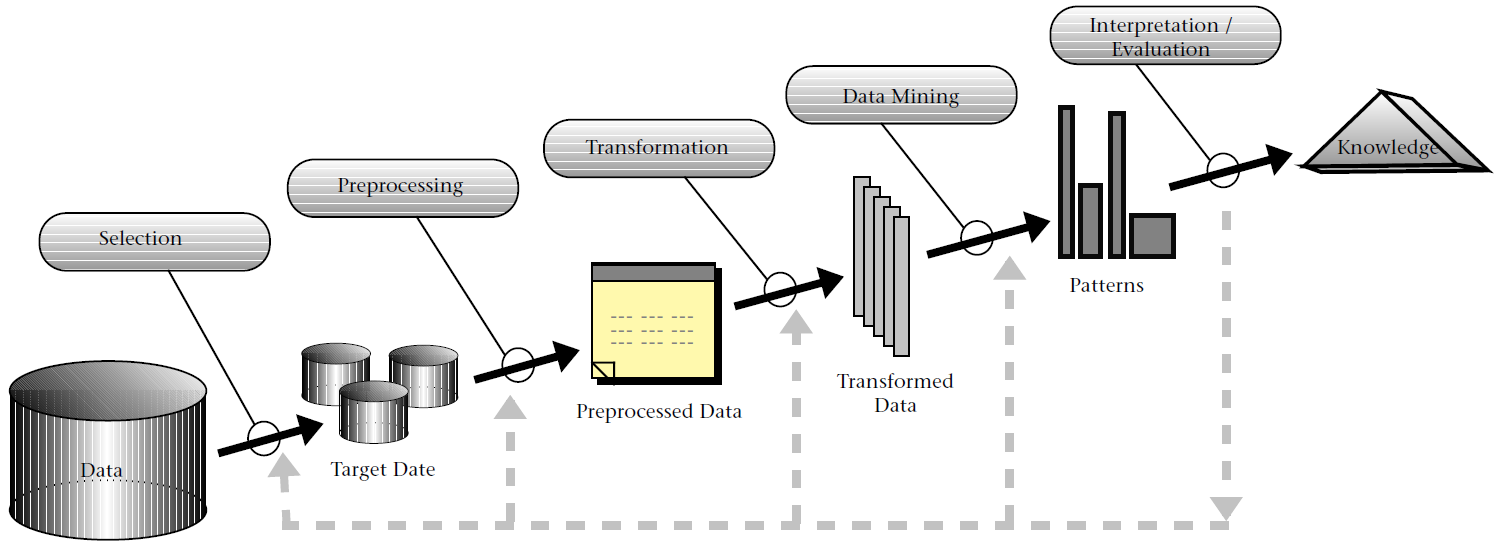
\includegraphics[width=\textwidth]{images/kddprocess}
\caption{Ein Überblick über die Schritte des KDD Prozesses nach \citep[S.~41]{fayyad_data_1996}}
\label{fig:kddprocess}
\centering
\end{figure}


\subsubsection{Selection}
Bevor der erste eigentliche Schritt, die Selektion der Daten, erfolgen kann, ist es unabdingbar, ein "Verständnis für das Anwendungsgebiet zu entwickeln".\citep[S.~42; eigene Übersetzung]{fayyad_data_1996} Ist das Verständnis hergestellt, kann ein "target data set"\citep[S.~42]{fayyad_data_1996} hergestellt werden. Dabei werden zuerst Daten aus unterschiedlichen - oft heterogenen - Quellen zusammengeführt und dann hinsichtlich des Ziels verdichtet.\citep[S.~70]{swamynathan_mastering_2017}

\subsubsection{Preprocessing}
Die verbleibende Teilmenge der ursprünglichen Daten muss nun noch gesäubert und für die nächsten Schritte vorbereitet werden. Dies geschieht, da unbereinigte Daten sowohl den Data Mining-Prozess verschlechtern können (unverlässliche oder falsche Ergebnisse), als auch die Zeit für das Mining deutlich verlängern können.\citep[S.~70]{swamynathan_mastering_2017}
Um die Qualität der Daten und des Mining zu verbessern, werden unter anderem folgende Aspekte betrachtet:\multicitep{fayyad_data_1996, S.~42; swamynathan_mastering_2017, S.~70}
\paragraph{Outliner treatment}\mbox{} \\
Ein Ausreißer (engl. outliner) kann beispielsweise ein "Extremer Wert in einer Variablen" oder ein "Extremer Wert des Residuums bei einer sinnvollen Regression"\citep[S.~25; Teil 5b]{hertle_datenanalyse_2016} sein. Ein Vorgehen für Ausreißer kann folgendermaßen aussehen (nach \citep[S.~25; Teil 5b]{hertle_datenanalyse_2016}):
\begin{enumerate}
\item Identifizieren der Ausreißer (evtl. durch eine erste Regression)
\item Interpretation im Sachzusammenhang (Messfehler oder wichtiger Teil der Population)
\item Entscheidung, ob man eine Regression der Daten mit oder ohne diese Ausreißer haben möchte
\item In der Darstellung der Ergebnisse auf die Ausreißer explizit eingehen und Vorgehen erläutern
\end{enumerate}

\paragraph{Noise removal}\mbox{} \\
Auch in einem Datensatz, der auf Ausreißer untersucht wurde, befinden sich immer noch unbekannte, unvollständige, falsche und fehlende Werte ("attribute noise"). Zusätzlich können Datenklassen falsch gekennzeichnet sein ("class noise"). Ist ein Datensatz von diesen Problemen betroffen, spricht man von "noisy data". Auf die Lösung dieses Problems wird an dieser Stelle nicht weiter eingegangen. 

\paragraph{Identifying duplicated values}\mbox{} \\
Wie oben angesprochen, wird der zu analysierende Datensatz aus mehreren Quellen zusammengeführt. Durch diesen Schritt können Datensätze doppelt (oder noch öfter) vorkommen. Das wird deutlich, wenn man folgendes Beispiel betrachtet: Über eine Kundenkarte werden Daten von Kunden eines Supermarkets je Filiale gespeichert. Bei einer überregionalen Kundenanalyse tauchen Kunden mehrfach auf, die in verschiedenen Filialen eingekauft haben. Hier ist anzumerken, dass doppelte Werte nicht zwangsläufig gelöscht werden müssen, sie sollten jedoch bei der Analyse bedacht werden.

\paragraph{Check for inconsistency}\mbox{} \\
Je größer ein Datensatz ist, umso wahrscheinlicher enthält der auch Inkonsistenzen \todo{quelle hierfür?}. Dies wird ebenfalls durch die Fusion von mehreren Quellen verstärkt (Beispiel: unterschiedliches Alter für einen Kundenstammsatz). Auch hier muss geprüft werden, wie mit diesen Werten umzugehen ist. Eventuell können Regeln festgelegt werden wie "immer der neuste Datenpunk ist der richtige".

\paragraph{Time series and changes}\mbox{} \\
Der letzte Punkt, der beim Preprocessing betrachtet werden muss, ist der Zusammenhang der Daten und dem Erfassungszeitpunkt. So können im Laufe der Zeit sich die Messmethodik (z.B. andere Sensoren), die Messgenauigkeit (z.B. bessere Sensoren) oder die Abstände der Messungen verändern.

\subsubsection{Transformation}
Der letzte Schritt vor dem eigentlichen Data Mining ist die Transformation. In diesem Prozessschritt geht es darum, "mit Dimensionsreduktions- oder -transformationsmethonden die effektive Anzahl an Variablen [...] zu reduzieren"\citep[S.~42; eigene Übersetzung]{fayyad_data_1996}. Dies geschieht beispielsweise durch das identifizieren und eliminieren invarianter Variablen. Ebenfalls wird versucht, solche Variablen zu finden, die mehrere Andere repräsentieren. Anschaulich dargestellt an einem Beispiel:
\begin{table}
\begin{tabular}{rrrrrrr}
  \hline
 & Person & Studium & ErfahrungExtern & ErfahrungIntern & Alter & Gehalt \\ 
  \hline
1 &   1 &   6 &   1 &   4 &  24 & 46450 \\ 
  2 &   2 &  18 &  30 &  15 &  55 & 85150 \\ 
  3 &   3 &  11 &   7 &   7 &  31 & 55900 \\ 
  4 &   4 &  11 &  15 &   8 &  36 & 63650 \\ 
  5 &   5 &  10 &   1 &  16 &  33 & 59050 \\ 
  6 &   6 &   6 &  25 &   6 &  38 & 68750 \\ 
  7 &   7 &  10 &  20 &  20 &  50 & 79000 \\ 
  8 &   8 &   7 &   0 &   1 &  23 & 43050 \\ 
   \hline
\end{tabular}
\caption{Einfacher Datensatz mit Berufserfahrung und Gehalt}
\label{tab:Beispiel_Berufserfahrung_R_output_simpleData}
\end{table}
Die Tabelle \ref{tab:Beispiel_Berufserfahrung_R_output_simpleData} zeigt einen einfachen Datensatz, in dem das Personal einer Firma und sein Gehalt festgehalten ist. "Studium" beschreibt Anzahl der Halbjahre im Studium. Analog dazu "ErfahrungExtern" und "ErfahrungIntern" die Berufserfahrung in Halbjahren. Zusätzlich ist das Alter der Personen gegeben.\newline
Führt man eine Regression (\ref{list:Regression1}) für den Datensatz durch (mit Studium, ErfahrungExtern, ErfahrungIntern, Alter als unabhängige und Gehalt als abhängige Variable), ergibt sich das Ergebnis in Tabelle \ref{tab:Regression1:output}.

\lstinputlisting[label=list:Regression1, caption=Einfache Regression mit allen Faktoren]{../R/Beispiel_Berufserfahrung/Regression1.R}

\begin{table}
\begin{tabular}{rrrrr}
  \hline
 & Estimate & Std. Error & t value & Pr($>$||) \\ 
  \hline
(Intercept) & 40000 & 1.415e-11 & 2827667776379022.00 & <2e-16 *** \\ 
  Studium & 300 & 5.167e-13 & 580659943804207.12 & <2e-16 *** \\ 
  ErfahrungExtern & 850 & 4.821e-13 & 1763103113756617.75 & <2e-16 *** \\ 
  ErfahrungIntern & 950 & 6.308e-13 & 1506009525690195.75 & <2e-16 *** \\ 
  Alter & 2.010e-13 & 8.103e-13 & 0.82 \\ 
   \hline
\end{tabular}
\caption{Output der einer einfachen Regression mit allen Variablen}
\label{tab:Regression1:output}
\end{table}

Ohne weiter auf die genauen 

\todo{hier weiter: ohne an dieser Stelle genauer auf die werte einzugehen, zeigt sich, dass...}
\todo{andere beispiele für trasnformation...smoothing, aggregation..."außer dem gerade verwendeten...blablabla" --> python buch}
\todo{weitere schritte aus Fayyad paper dann...}

\subsubsection{Data Mining}
Fifth is matching the goals of the KDD process (step 1)
Sixth is exploratory analysis and model and hypothesis selection
Seventh is data mining

\subsubsection{Interpretation/Evaluation}
Eighth is interpreting mined patterns
Ninth is acting on the discovered knowledge:


\subsection{CRoss Industrial Standard Process for Data Mining (CRISP – DM)}
\subsection{Sample, Explore, Modify, Model and Assess (SEMMA)}
\subsection{Auswahl}




\section{Data Mining (Prozess)}
Data mining Prozess beschreiben und die Stufen von Zeile etc. Bis zur Interpretation 
\subsection{Ziele}
\subsection{Datenauswahl}
\subsection{Datenbereinigung}
\subsection{Datenreduktion (Transformaton)}
\subsection{Modellauswahl}
\subsection{Data-Mining (Datenanalyse)}
\subsection{Interpretation}
\section{Machine Learning } 
\subsection{Supervised...}
Man weiß, nach was man sucht…
\subsubsection{Decision Tree}
\subsubsection{Neares Neighbour}
\subsubsection{Random Forest}
\subsubsection{SVM}
\subsection{Unsupervised...}
\subsubsection{K means}
\subsubsection{Hierarchical clustering}
\subsubsection{Neuronal networks}
\subsubsection{...}
Man sucht nur cluster/gruppen/etc
\section{Krypotwährung(en)}
Bitcoin,ethereum, litecoin, dogecoin; auswahl hier nur 1/2
\section{Saas}
\section{Microsoft Azure ML Studio}
\subsection{Allgemeine Beschreibung}
\subsection{Aufbau }
\subsubsection{Projects}
\subsubsection{Experiments}
\subsubsection{Web Services}
\subsubsection{Notebooks}
\subsubsection{Datasets}
\subsubsection{Trained Models}
\subsubsection{Settings}
\subsection{Elemente}
relevate auswählen
\subsubsection{Saved Datasets}
\subsubsection{Data Transformation Conversations}
\subsubsection{Data Transformation}
\subsubsection{Data Input and Output}
\subsubsection{Feature Selection}
\subsubsection{Machine Learning}
\subsubsection{OpenCV Library Models}
\subsubsection{Python Language Model}
\subsubsection{R Language Model}
\subsubsection{Statistical Functions}
\subsubsection{Text Analysis}
\subsubsection{Time Series Anomaly Detection}
\subsubsection{Web Service}
